\documentclass[12pt, twoside]{article}
\usepackage[letterpaper, margin=1in, headsep=0.5in]{geometry}
\usepackage[english]{babel}
\usepackage[utf8]{inputenc}
\usepackage{amsmath}
\usepackage{amsfonts}
\usepackage{amssymb}
\usepackage{tikz}
\usetikzlibrary{quotes, angles}
\usepackage{graphicx}
\usepackage{enumitem}
\usepackage{multicol}
\usepackage{hyperref}

\newif\ifmeta
\metatrue %print standards and topics tags

\title{IB Mathematics}
\author{Chris Huson}
\date{January 2022}

\usepackage{fancyhdr}
\pagestyle{fancy}
\fancyhf{}
\renewcommand{\headrulewidth}{0pt} % disable the underline of the header
\raggedbottom


\fancyhead[LE]{\thepage}
\fancyhead[RO]{\thepage \\ Name: \hspace{4cm} \,\\}
\fancyhead[LO]{BECA / IB Math 03-Quadratic functions\\* 28 January 2022}

\begin{document}

\subsubsection*{4.7 Classwork: Direct and inverse variation}
\begin{enumerate}
\item The functions $f(x)=x^3-0.5x^2-3x+1$ and $g(x)=0.5x+2$ are defined over the domain $[-2,1]$ as shown on the grid below. Find the two points where $f(x)=g(x)$. (the intersections)
    \begin{center}
      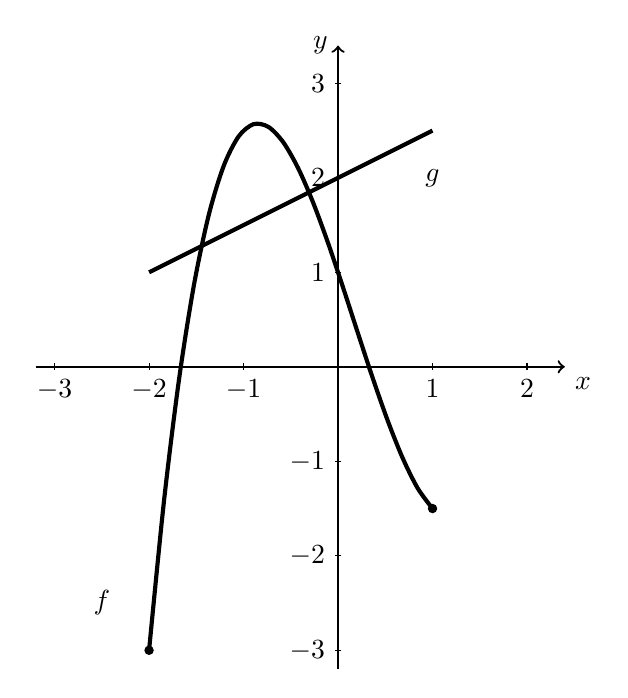
\begin{tikzpicture}[scale=1.2]
        %\draw [help lines] (-3,-3) grid (3,4);
        \draw [thick, ->] (-3.2,0) -- (2.4,0) node [below right] {$x$};
        \draw [thick, ->] (0,-3.2)--(0,3.4) node [left] {$y$};
        \foreach \x in {-3,-2,-1,1,2} \draw (\x cm,1pt) -- (\x cm,-1pt) node[anchor=north] {$\x$};
        \foreach \y in {-3,-2,-1,1,2,3} \draw (1pt,\y cm) -- (-1pt,\y cm) node[left] {$\y$};
        %\draw [thick] (-2,0) -- (0,4) -- (3,5);
        \draw [line width=1.5pt,smooth,samples=20,domain=-2:1] plot(\x,\x^3-0.5*\x*\x-3*\x+1);
        \draw [line width=1.5pt,smooth,samples=20,domain=-2:1] plot(\x,0.5*\x+2);
        \fill (-2,-3) circle[radius=0.05];
        %\fill (-0.85,2.58) circle[radius=0.1] node [left]{$(-0.75,2.6)$};
        \node at (-2.5,-2.5){$f$};
        \node at (1,2){$g$};
        \fill (1,-1.5) circle[radius=0.05];
      \end{tikzpicture}
    \end{center}

\item An inverse function of the form $\displaystyle f(x)=\frac{1}{x+p}+q$ is shown on the grid below. 
    \begin{multicols}{2}
        \begin{enumerate}[itemsep=1cm]
            \item Write down the equation of the horizontal asymptote.
            \item  Write down the equation of the vertical asymptote.
            \item Hence, write down $p$ and $q$.
            \item Find $f(0)$.
            \item Solve for $x$ such that $f(x)=0$.
        \end{enumerate}
        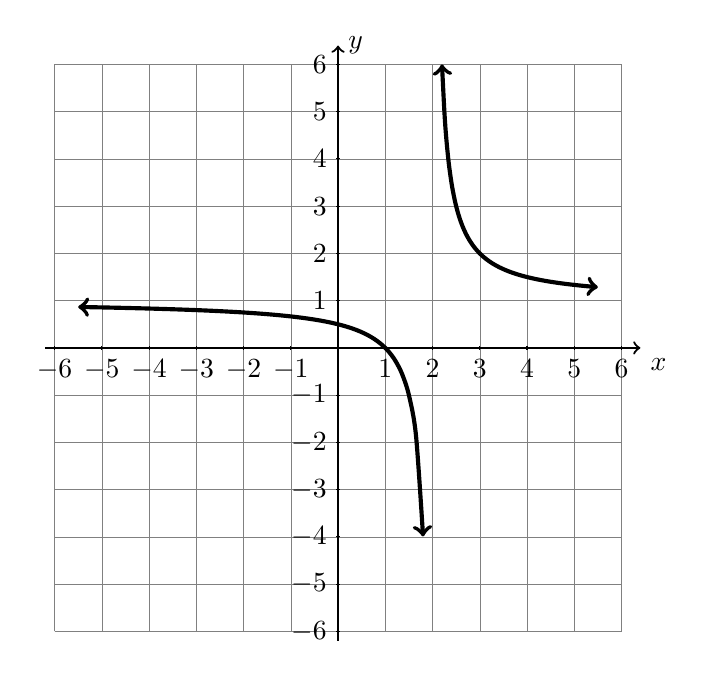
\begin{tikzpicture}[scale=0.6]
        \draw [help lines] (-6,-6) grid (6,6);
        \draw [thick, ->] (-6.2,0) -- (6.4,0) node [below right] {$x$};
        \draw [thick, ->] (0,-6.2)--(0,6.4) node [right] {$y$};
        \foreach \x in {-6,...,-3,-2,-1,1,2,...,6} \draw (\x cm,1pt) -- (\x cm,-1pt) node[anchor=north] {$\x$};
        \foreach \y in {-6,...,-3,-2,-1,1,2,...,6} \draw (1pt,\y cm) -- (-1pt,\y cm) node[left] {$\y$};
        \draw [<->,line width=1.5pt,smooth,samples=50,domain=-5.5:1.8] plot(\x,{1/(\x-2)+1});
        \draw [<->,line width=1.5pt,smooth,samples=50,domain=2.2:5.5] plot(\x,{1/(\x-2)+1});
        \end{tikzpicture}
    \end{multicols}

\newpage
\item A cardboard box manufacturing company is building boxes with length represented by $x+1$, width by $5-x$, and height by $x-1$. The volume of the box is modeled by the function below.
\begin{multicols}{2}
    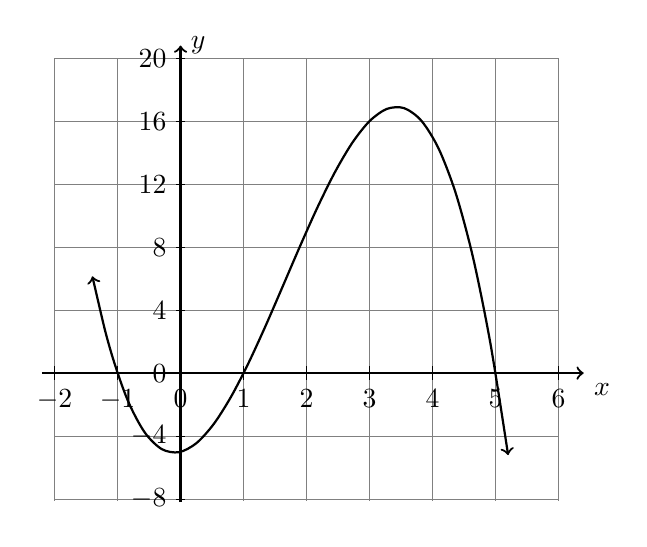
\begin{tikzpicture}[x=1cm, y=0.25cm, scale=0.8]
        \draw [help lines] (-2,-8.1) grid (6,20);
        \draw [thick, ->] (-2.2,0) -- (6.4,0) node [below right] {$x$};
        \draw [thick, ->] (0,-8.2)--(0,20.8) node [right] {$y$};
        \foreach \x in {-2,...,6}
            \draw[shift={(\x,0)}] (0,3pt)--(0,-3pt) node[below] {$\x$};
        \foreach \y in {-8,-4,...,20}
            \draw[shift={(0,\y)}] (2pt,0pt)--(-2pt,0pt) node[left]  {$\y$};
        \draw [<->,thick,smooth,domain=-1.4:5.2] plot(\x,{-(\x)^3+5*(\x)^2+(\x)-5});
    \end{tikzpicture}
\begin{enumerate}[itemsep=0.75cm]
    \item Over what interval of positive $x$ values is the volume positive?
    \item Estimate the maximum possible volume of the box.
    \item Approximately the value of $x$ would maximize the volume of the box.
\end{enumerate} 
\end{multicols}
%\vspace{0.5cm}

\item Shown in the plot below is the function $f(x)=x^3+4x^2-1x-4$.
\begin{enumerate}
    \item Write down the value of $f(0)$. On the graph, mark the point for $f(0)$ with a star.\vspace{0.75cm}
    \item Write down the solutions to $f(x)=0$. Mark them with ``X'' marks on the graph.\vspace{0.75cm}
    \item Mark the portion of the function that is \emph{decreasing} with a squiggly line.
\end{enumerate}
\begin{center}
    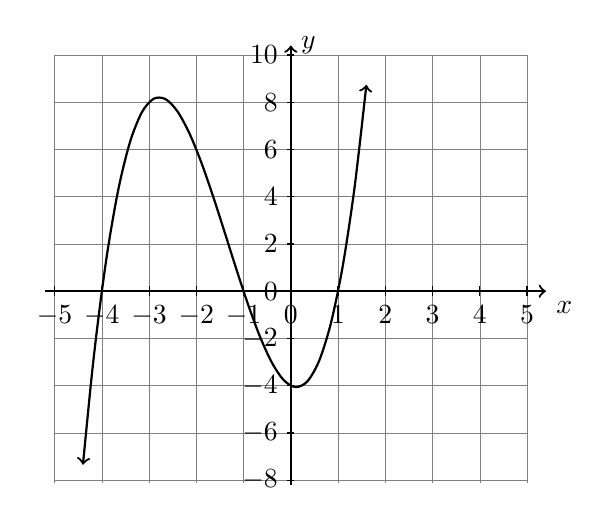
\begin{tikzpicture}[x=1cm, y=0.5cm, scale=0.6]
        \draw [help lines] (-5,-8.1) grid (5,10);
        \draw [thick, ->] (-5.2,0) -- (5.4,0) node [below right] {$x$};
        \draw [thick, ->] (0,-8.2)--(0,10.4) node [right] {$y$};
        \foreach \x in {-5,...,5}
            \draw[shift={(\x,0)}] (0,3pt)--(0,-3pt) node[below] {$\x$};
        \foreach \y in {-8,-6,...,10}
            \draw[shift={(0,\y)}] (2pt,0pt)--(-2pt,0pt) node[left]  {$\y$};
        \draw [<->,thick,smooth,domain=-4.4:1.6] plot(\x,{(\x)^3+4*(\x)^2-(\x)-4});
    \end{tikzpicture}
\end{center}

\end{enumerate}
\end{document}



